\section{Contexto de trabajo}

Actualmente vivimos en un entorno que dominado por la tecnología. Día a día se desarrollan nuevas herramientas con el fin de ayudar al ser humano a realizar tareas de una forma más fácil y eficiente, como los HMD (Head-mounted Display)\cite{B15}.


Por otro lado también nos encontramos en una época donde el diseño es un área de gran importancia en cualquier sector del mercado, por ejemplo, un buen diseño web en un sitio es fundamental lograr que un producto se logre vender o difundir, un buen diseño gráfico en campañas de marketing asegura más clientes; de igual forma nos encontramos con el diseño de interiores. Para ésta última área se suelen contratar diseñadores de interiores profesionales para lograr que los espacios interiores de un inmueble consigan tal armonía que mejoren la calidad de vida de quienes lo habitan y además generen un impacto en las personas que usan éstas habitaciones.\par
El diseño de interiores no tiene un proceso estandarizado, sin embargo a nivel general, debe seguir el siguiente flujo: un cliente acude con un diseñador de interiores profesional quien acude a su domicilio para revisar los espacios interiores del inmueble, y conocer las necesidades y presupuesto del cliente. Con base en esta información, el diseñador elabora una propuesta de actividades donde se describen con detalles las actividades que van a involucrar el diseño de interiores así como la fecha en la que serán realizadas, también elabora una propuesta de diseño donde le muestra al cliente cómo se vería el resultado final, la cual puede ser a través de modelados 3D, o imágenes con fotomontajes. Cuando el cliente acepta ambas propuestas, el diseñador se dispone a realizar la obra hasta finalizarla.\par
El proceso anteriormente descrito se puede observar en las figuras 1.1, 1.2, 1.3 y 1.4 a través de un modelo de proceso de negocio.\par
Teniendo a la mano una gran diversidad de herramientas tecnológicas, podemos usar estos elementos para lograr que el diseño de interiores sea más sencillo, intuitivo y más rápido, y que cualquier persona pueda realizarlo sin tener todos los conocimientos y habilidades que se requieren para ello o para que un diseñador de interiores pueda hacerlo de forma más fácil y rápida.
\newpage

\begin{figure}[!htbp]
	\centering
	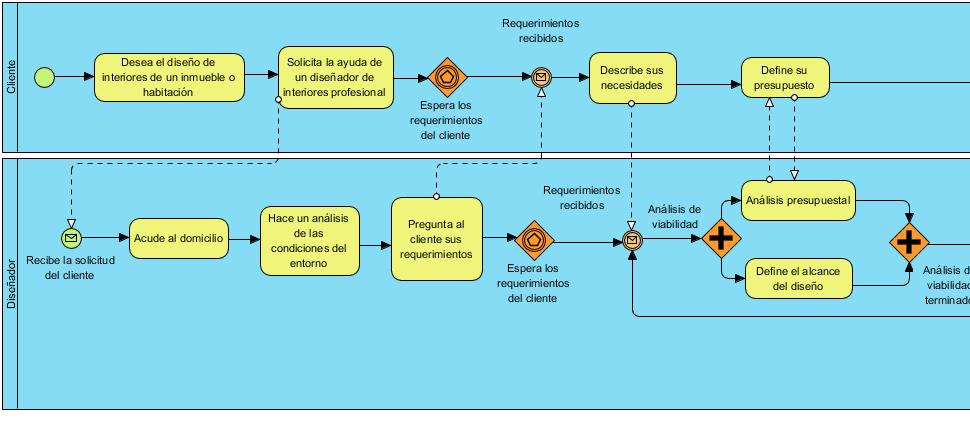
\includegraphics[width=16cm]{imagenes/marcoteorico/diseno_01.jpg}
	\caption{Modelo del proceso de diseño de interiores.}
	\label{fig:bpmn_antes}
\end{figure}
\begin{figure}[!htbp]
\centering
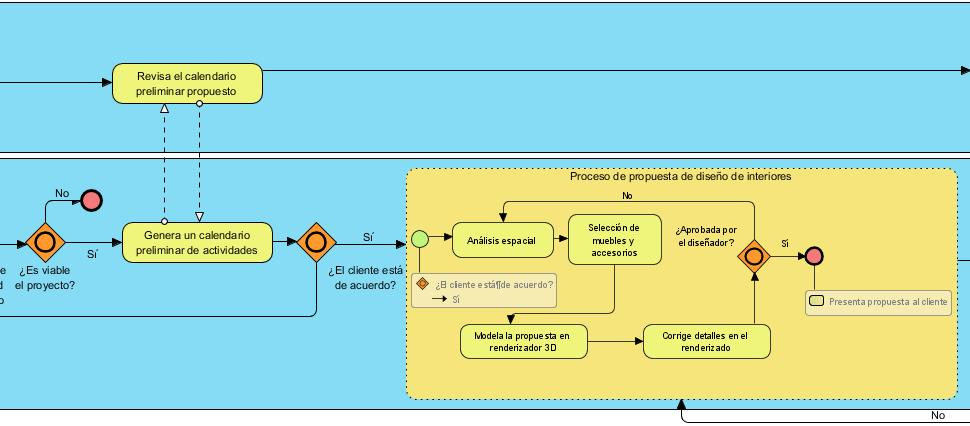
\includegraphics[width=16cm]{imagenes/marcoteorico/diseno_02.jpg}
\caption{Modelo del proceso de diseño de interiores.}
\label{fig:bpmn_antes}
\end{figure}
\begin{figure}[!htbp]
\centering
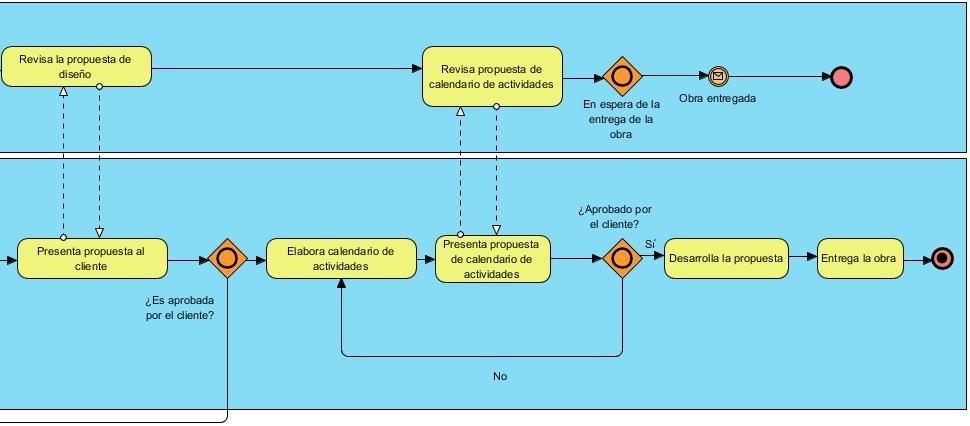
\includegraphics[width=16cm]{imagenes/marcoteorico/diseno_03.jpg}
\caption{Modelo del proceso de diseño de interiores.}
\label{fig:bpmn_antes}
\end{figure}
